\newpage
\section{Matter Waves}

\subsection{Mystery of the Light Wave}
\subsubsection{A Fundamental Mystery}
How light can be a wave (which spreads out over a region) in classical physics but be emitted and absorbed as photons (which originate and vanish at points) in quantum physics? 

\subsubsection{Light as a Probability Wave}
Double-slit experiments tell us
\begin{enumerate}
    \item Light is generated in the source as photons, 
    \item absorbed in the detector as photons, and
    \item travels bewteen source and detector as a probability wave. 
\end{enumerate}

The \highlight{probability density} of detecting a photon at some point $P$ in space depends on the irradiance $I\varpropto E_0^2$ at that point. Thus, the net $E_0$ at $P$ can be interpreted as the \highlight{probability amplitude}. To go further, one will need quantum electrodynamics(QED), the quantum theory of the interaction of light and matter. 


\subsection{Electrons and Matter Waves}
\subsubsection{De Broglie Hypothesis}
A beam of light is a wave, but it transfers energy and momentum to matter only at points, via photons. Electron is a particle with energy and momentum. We can think of a beam of moving electron --- or any other particle --- as a matter wave. De Broglie proposed that one could assign a wavelength $\lambda$ to a particle with momentum of magnitude $p$. Like that of photons, we define
\begin{align*}
    \lambda=&\frac{h}{p}\\
    =&\frac{h}{mv}=\frac{h}{m_0 v}\sqrt{1-\frac{v^2}{c^2}}\\
    \text{When }v \ll c,\,\lambda=&\frac{h}{m_0 v}
\end{align*}
which is known as the \highlight{de Broglie wavelength} of the moving particle. 

\subsubsection{Electron Diffraction}
Both X rays and electrons are waves.

\subsubsection{The Interference of Electrons}
In a more recent experiment, an interference pattern was built up when electrons were sent, one by one, through a double-slit apparatus. When an electron hit the viewing screen, it caused a flash of light whose position was recorded. Repeat the experiment at such low intensity that at any given time there is just one particle in the interference region. 

\begin{figure}[H]
    \centering
    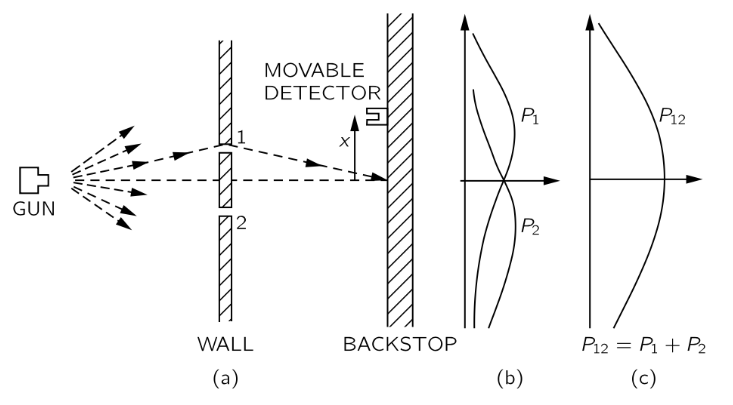
\includegraphics[width=0.309\textwidth]{Lec22/Newtonian Physics}
    \caption{Newtonian Physics}
\end{figure}

In Newtonian physics, a particle is only aware of the slit through which it goes, it has no idea how many other slits are open or closed or even exist. Therefore, when both slits are open, $P_{12}=P_1+P_2$. 

\subsubsection{Matter Wave}

\begin{figure}[H]
    \centering
    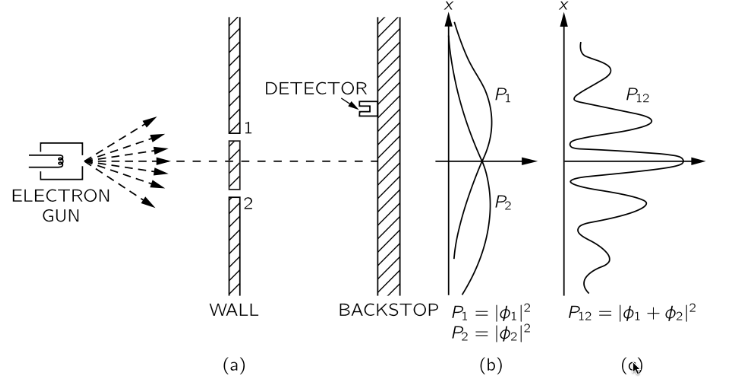
\includegraphics[width=0.309\textwidth]{Lec22/Matter Wave}
    \caption{Matter Wave}
\end{figure}


The electrons arrive in lumps, like particles, and the probability of arrival of these lumps is distributed like the distribution of intensity of a wave. 

It is in this sense that an electron behaves \highlight{sometimes like a particle and sometimes like a wave}. Our rescue, of course, come from optics, where light or photons also interfere. There, we need to add amplitude $A$, rather than intensity $|A|^2$. Similarly here, the experimental observation forces us to introduce the \highlight{probability amplitude $\psi$} which is a complex number. The probability of an event in an ideal experiment is then given by $|\psi|^2=\psi * \psi$. 

When an event can occur in several alternative ways, the probability amplitude for the event is the \highlight{sum of the probability amplitudes} for each way considered separately. 
\begin{align*}
    \psi=\psi_1+\psi_2+\cdots
\end{align*}
The probability for the event is, 
\begin{align*}
    P=|\psi|^2=|\psi_1|^2+|\psi_2|^2+2\mathfrak{R} (\psi_1^{\dagger}\psi_2)+\cdots
\end{align*}
The interference term $2\mathfrak{R} (\psi_1^{\dagger}\psi_2)$ is responsible for the rapid oscillations in the experiment. 

\begin{figure}[H]
    \centering
    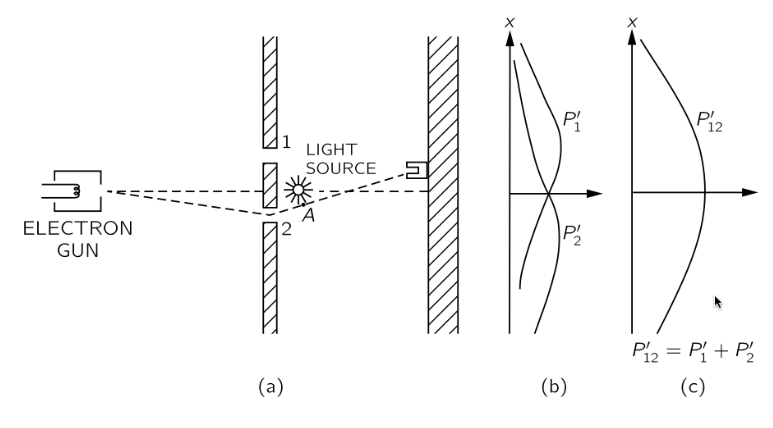
\includegraphics[width=0.309\textwidth]{Lec22/The Which-Way Experiment}
    \caption{The Which-Way Experiment}
\end{figure}


Not weird enough? Now, if an experiment is performed which is capable of determining whether one or another alternative is actually taken, the interference is lost. The experiment tells us that the probability of the event in the which-way experiment is the sum of the probabilities for each alternative,
\begin{align*}
    P=|\psi|^2=|\psi_1|^2+|\psi_2|^2
\end{align*} 
just as what happens in the classical case. Thus an electron acts like it went through one particular slit if we see it doing that and acts like it did not have a specific path (through a specific slit) when it is not seen.

To see an electron with a resolution comparable to slit separation $d$, (so we know which slit it took) requires light with $\lambda < d$, this is just standard wave theory. But, the light is made of photons each with momentum $p > \frac{h}{d}$. So measuring the position of the electron has made us disturb its momentum. The amount of momentum transferred to the electron in the act of observation is indefinite.This is a manifestation of \highlight{Heisenberg’s uncertainty principle}, which says you cannot measure the momentum and coordinate of a particle simultaneously to arbitrary accuracy.

\subsection{Heisenberg’s Uncertainty Principle}

The probabilistic nature of quantum physics places an important limitation on detecting a particle’s position and momentum. That is, it is not possible to measure the position $\vec{r}$ and the momentum $\vec{p}$ of a particle simultaneously with unlimited precision. The uncertainties
in the components of these quantities are given by
\begin{align*}
    \Delta x\cdot \Delta p_x \ge \hbar\\
    \Delta y\cdot \Delta p_y \ge \hbar\\
    \Delta z\cdot \Delta p_z \ge \hbar
\end{align*}

They are due to the fact that electrons and other particles are matter waves and that repeated measurements of their positions and momenta involve \highlight{probabilities, not certainties}. In the statistics of such measurements, we can view, say, $\Delta x$ and $\Delta p_x$ as the spread (actually, the standard deviations) in the measurements. Couldn’t we very precisely measure $p_x$ and then next very precisely measure $x$ wherever the electron happens to show up? Doesn’t that mean that we have measured both $p_x$ and $x$ simultaneously and very precisely? No, the flaw is that although the first measurement can give us a precise value for $p_x$ , the second measurement necessarily alters that value. 

What form does the electron wave function have? The naive guess could be sin kx , or cos kx . But they have spatial variance that is inconsistent with our intuition. To represent the electron by a wave, we need a function, which is called \highlight{wave function}, with a wavelength $\lambda=\frac{2\pi}{k}$, but its square should not show any variation in $x$, i.e.
\begin{align*}
    \psi(x)=e^{i(kx-\omega t)}
\end{align*}

If we measure $p_x$ now, we obtain $p_x=\hbar k$ without uncertainty, but the particle exists anywhere with the same probability, $\Delta x=\infty$.

If we measure $x$ then, we will find the electron somewhere at $x_0$. Once we find it, it can't be elsewhere. So the wave function suddenly \highlight{collapses} to
\begin{align*}
    \psi(x)=\delta(x-x_0)
\end{align*}
Now, the Fourier transform of the $\delta$-function tells us 
\begin{align*}
    \bar{\psi}(p)=\mathcal{F} (\psi(x))=constant
\end{align*}
In this case, $\Delta x=0$ but $\Delta p=\infty$. 

The major significance of the \highlight{wave-particle duality} is that all behavior of light and matter can be explained through the use of a \highlight{complex wave function $\psi(x,y,z,t)$}. The probability of finding a particle somewhere at a particular time is proportional to
\begin{align*}
    P(x,y,z,t)=\psi^{\dagger}(x,y,z,t)\psi(x,y,z,t)
\end{align*}
It turns out that the wave function satisfies a differential equation, known as Schroedinger's equation.